\documentclass[11pt,a4paper]{ctexart}
\usepackage{fontspec}
\defaultfontfeatures{Mapping=tex-text}
\usepackage{xunicode}
\usepackage{xltxtra}
%\setmainfont{???}
\usepackage{amsmath}
\usepackage{amsfonts}
\usepackage{amssymb}
\usepackage{graphicx}
\usepackage{amsthm}
\usepackage{array}
\usepackage{float}   %{H}
\usepackage{booktabs}  %\toprule[1.5pt]
\usepackage[titletoc]{appendix}
%===================%插入代码需要的控制
\usepackage{listings}
\usepackage{xcolor}
\lstset{
	numbers=left, 
	numberstyle= \tiny, 
	keywordstyle= \color{ blue!70},
	commentstyle= \color{red!50!green!50!blue!50}, 
	frame=shadowbox, % 阴影效果
	rulesepcolor= \color{ red!20!green!20!blue!20} ,
	escapeinside=``, % 英文分号中可写入中文
} 
%===================%
\usepackage[left=2cm,right=2cm,top=2cm,bottom=2cm]{geometry}

\newtheorem{theorem}{定理}
\newtheorem{definition}{定义}
\newtheorem*{solution}{解}
\newtheorem{practice}{题}
\newcommand{\Sum}[3][i]{\sum\limits_{#1=#2}^{#3}}
\newcommand{\Int}[2]{\int_{#1}^{#2}}
\newcommand{\Sample}[3][X]{{#1}_{#2},\dotsi ,{#1}_{#3}}
\newcommand{\Samiid}[4][X]{{#1}_{#2},\dotsi ,{#1}_{#3}~iid\backsim {#4}}
\newcommand{\norm}[1]{\left\Vert #1\right\Vert_{\infty}}
\newcommand{\diff}[3]{\frac{\partial^{#3}{#1}}{\partial {#2}^{#3}}}
\newcommand{\abs}[1]{\left| {#1}\right|}
\newcommand{\normdis}[2]{N(#1,{#2}^2)}

\title{Time Series HomeWork (1)}
\author{钟瑜 \quad 222018314210044}
\date{\today}
\begin{document}
\maketitle

\begin{enumerate}
%================================================================%	
	
\item[1.]附录B中的B6是1973至1978年美国在意外事故中的死亡人数。

利用至少两种方法对该时间序列进行分解。要求如下:

(1)画出数据图,给出数据的周期T;\\
(2)给出趋势项、季节项和随机项的计算公式;\\
(3)画出趋势项、季节项和随即项的数据图;\\
(4)对1979年的意外死亡人数做出预测。
\begin{solution}
	
\vspace{3ex}

数据图如下:
\begin{figure}[H]
	\centering
	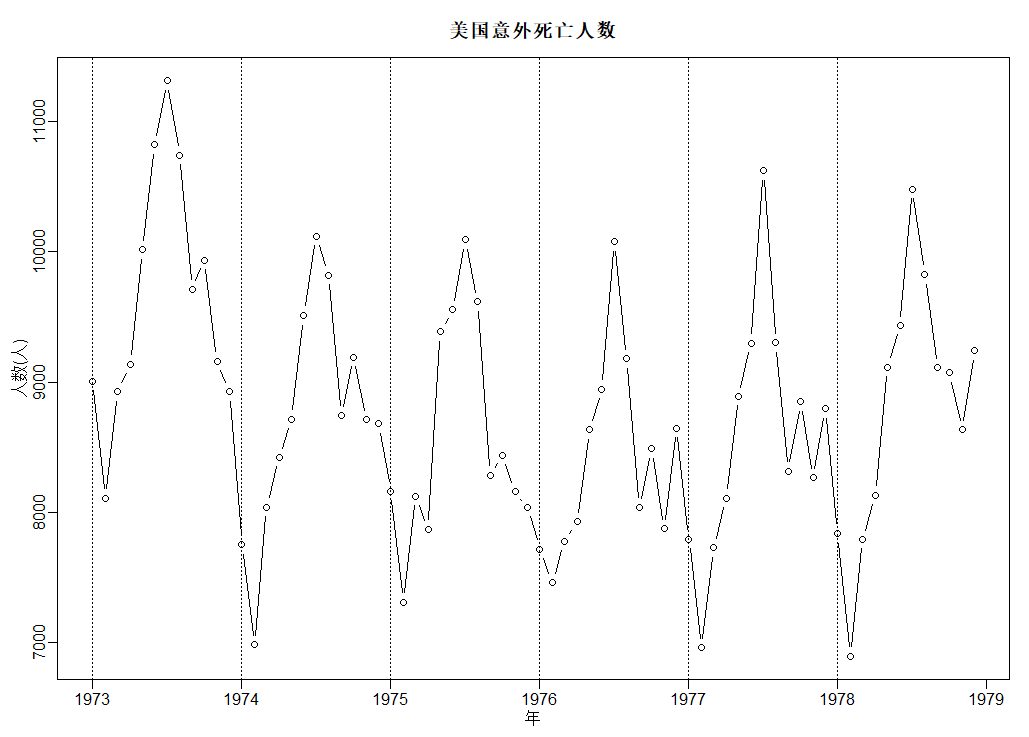
\includegraphics[width=12cm]{1.png}  
	\caption{美国意外死亡人数}
\end{figure}
显然如图可知,数据的周期为12个月。

\begin{itemize}
	\item \textbf{方法一:分段趋势}
	
趋势项$\left\lbrace T_t\right\rbrace $定义成年平均值,公式如下
\begin{equation}
T_t=T(t) =\left\{
\begin{aligned}
\frac{\sum_{j=1}^{12}c_j}{12} , t &=1,...,12 \\
\frac{\sum_{j=13}^{24}c_j}{12}, t &=13,...,24 \\
...\\
\frac{\sum_{j=61}^{72}c_j}{12}, t &=61,...,72 \\
\end{aligned}
\right.
\end{equation}

\begin{equation}
=\left\{
\begin{aligned}
8982.083333 , t &=1,...,12 \\
8723.75, t &=13,...,24 \\
8585.833333, t &=25,...,36 \\
8396.75, t &=37,...,48 \\
8576.833333, t &=49,...,60 \\
8796.75,t &=61,...,72 \\
\end{aligned}
\right.
\end{equation}
其中$c_j$表示第j个月的死亡人数;用第k个月的平均值作为季节项
$S(k),1\leq k\leq12$
的估计.用$x_{j,k}$,$T_{j,k}$分别表示第j年第k个月的数据和趋势项,则时刻(j,k)的时间次序指标为$k+12(j-1)$
\begin{equation}
\begin{aligned}
	S(k)&=\frac{1}{6}\sum_{j=1}^{6}(x_{j,k}-T_{j,k})\\
	&=\frac{1}{6}\sum_{j=0}^{5}(x_{k+12j}-T_{k+12j}),1\leq k\leq12
\end{aligned}
\end{equation}

计算结果如下

\begin{table}[H]   %[H]
	\centering
	\begin{tabular}{c}
		\toprule[1.5pt]
		$S(k)$  \\
		\midrule[1pt]
		-744.61111 \\
		-1504.77778 \\
		 -724.77778 \\
		  -523.77778 \\
		    337.55556 \\
		      806.72222\\
	 1664.22222 \\
	   960.55556  \\
	    -88.27778 \\
	      206.55556 \\
	       -321.44444 \\
	         -67.94444\\
		\bottomrule[1.5pt]
	\end{tabular}
\end{table}


下图为原始序列、趋势、拟合(包括趋势与季节项):
\begin{figure}[H]
	\centering
	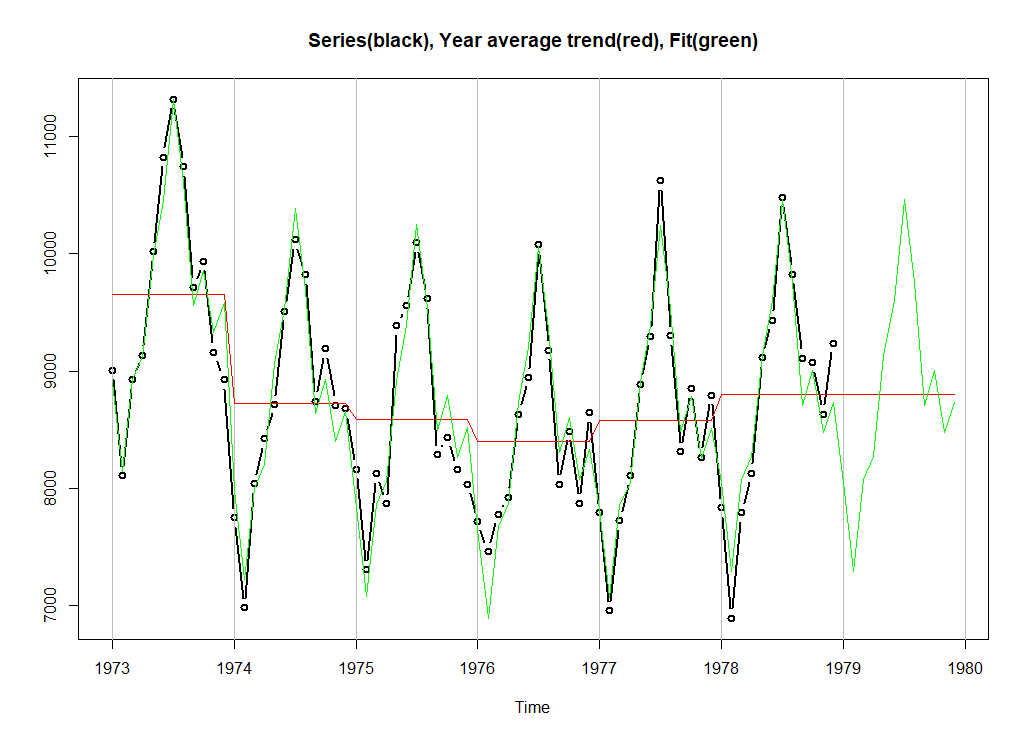
\includegraphics[width=12cm]{2.png}  
	\caption{原始序列、趋势、拟合(包括趋势与季节项)}
\end{figure}
最后,随机项的计算公式
\begin{equation}
R_t=x_t-T_t-S_t,1\leq t\leq72
\end{equation}


下图为去掉了趋势后的序列、季节项、取掉了趋势与季节项后的随机项:
\begin{figure}[H]
	\centering
	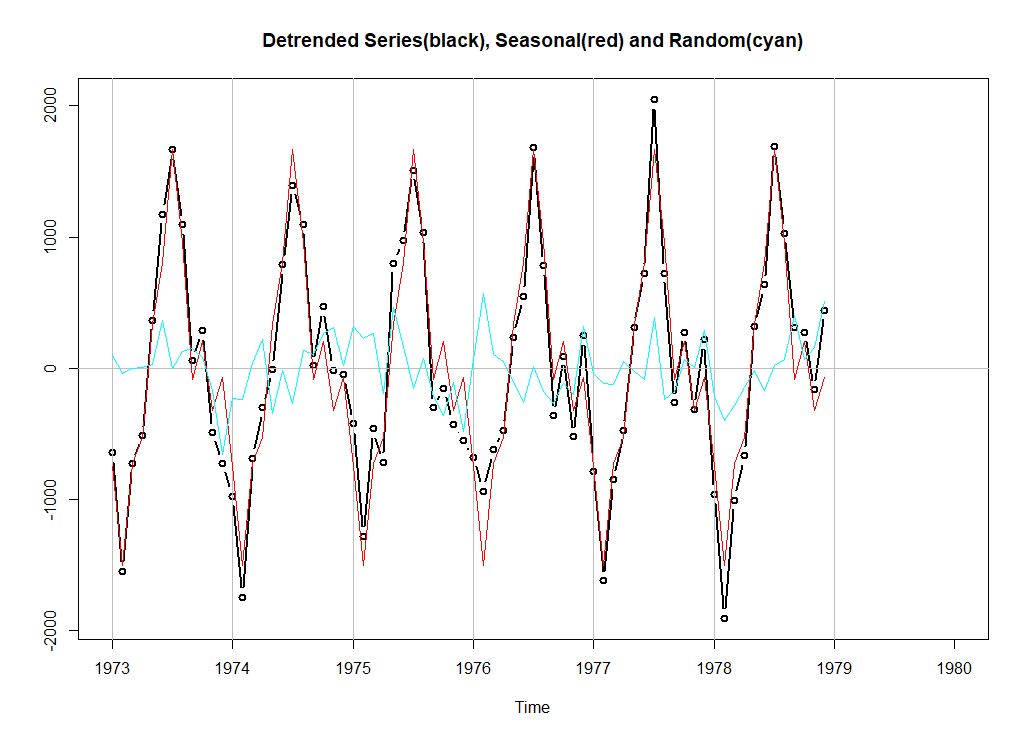
\includegraphics[width=12cm]{3.png}  
	\caption{去掉了趋势后的序列、季节项、取掉了趋势与季节项后的随机项}
\end{figure}


	\item \textbf{方法二:回归直线趋势}
	
趋势项用回归直线表示,这时认为$(x_t,t)$满足一元线性回归模型
\begin{equation}
x_t=a+bt+\epsilon_t,t=1,...,72
\end{equation}
定义
\[
\mathbf{X} = \left(
\begin{array}{cccc}
	x_{1} & x_{2} & \ldots & x_{72}
\end{array} \right)^T,
\]
\[
\mathbf{Y} = \left(
\begin{array}{cccc}
1 & 1 & \ldots & 1\\
1 & 2 & \ldots & 72\\
\end{array} \right),
\]
\[
\mathbf{\epsilon} = \left(
\begin{array}{cccc}
\epsilon_{1} & \epsilon_{2} & \ldots & \epsilon_{72}
\end{array} \right)^T,
\]

$(a,b)^T$的最小二乘估计由公式$$(a,b)^T=(YY^{T})^{-1}YX$$决定,用r计算得
$$a=9099.17$$$$b=-8.51$$
回归方程为
\begin{equation}
x_t=9099.17+-8.51t
\end{equation}
趋势项$\left\lbrace T_t\right\rbrace $的估计值是回归直线$$T_t=9099.17+-8.51t$$

下图绘制了原始数据、估计的趋势、拟合值(包括趋势与季节项):
\begin{figure}[H]
	\centering
	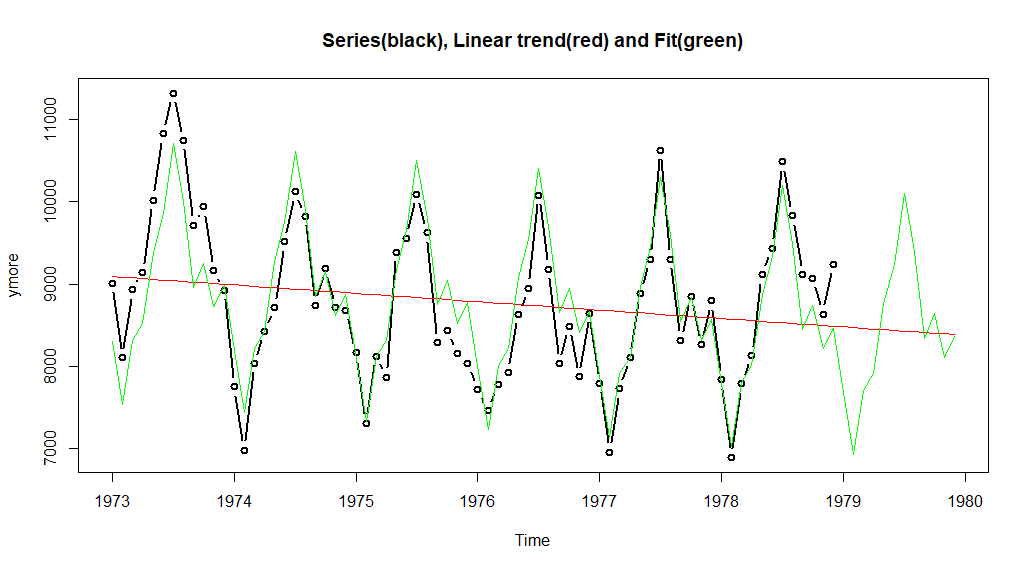
\includegraphics[width=12cm]{4.png}  
	\caption{原始数据、估计的趋势、拟合值(包括趋势与季节项)}
\end{figure}
利用原始数据$\left\lbrace x_t\right\rbrace $减去趋势项的估计$\left\lbrace T_t\right\rbrace $后得到的数据基本只含有季节项和随机项。我仍用第k月的平均值作为季节项$S(k)$的估计。利用方法一的公式计算结果如下


\begin{table}[H]   %[H]
 \centering
\begin{tabular}{c}
\toprule[1.5pt]
$S(k)$  \\
\midrule[1pt]
-791.40798\\
 -1543.06612  \\
 -754.55760 \\
  -545.04908 \\
   324.79277\\
 802.46796 \\
  1668.47648  \\
   973.31834 \\
     -67.00647 \\
       236.33538\\
 -283.15610  \\
  -21.14758\\
\bottomrule[1.5pt]
\end{tabular}
\end{table}
最后,随机项的计算公式
\begin{equation}
R_t=x_t-T_t-S_t,1\leq t\leq72
\end{equation}
\begin{figure}[H]
	\centering
	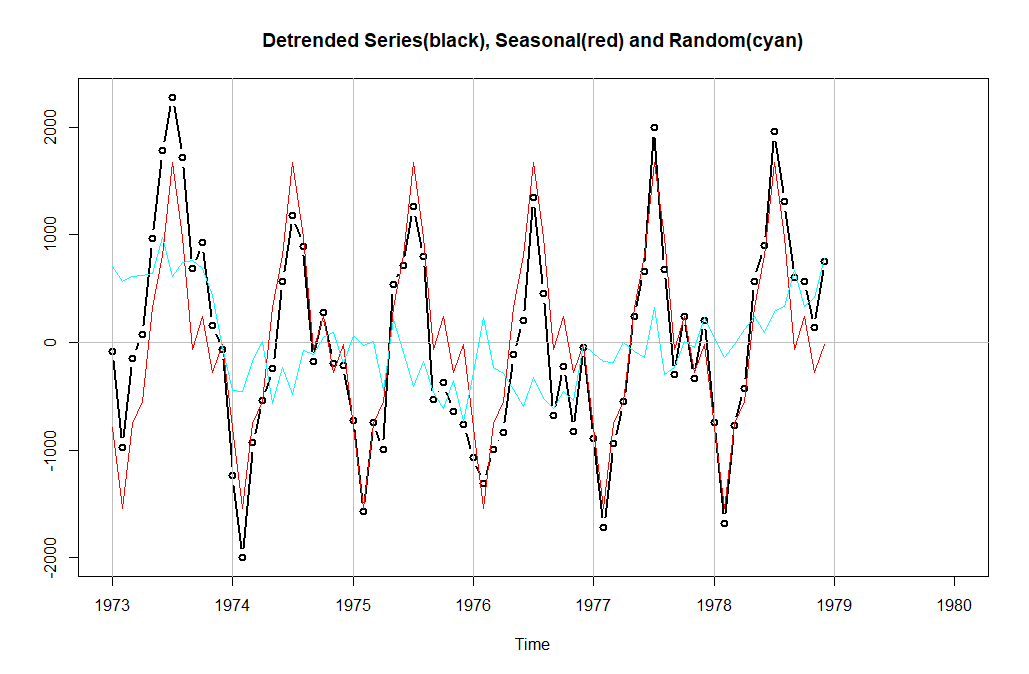
\includegraphics[width=12cm]{5.png}  
	\caption{去掉了趋势后的序列、季节项、取掉了趋势与季节项后的随机项}
\end{figure}

\end{itemize}




\end{solution}
%=================================================================%
\end{enumerate}
\centering\textbf{\Large 附录}


\begin{appendices}
	
\section{数据图}
\begin{lstlisting}[language=r]
B6.siwangrenshu <-
ts(c(
1973,9007,8106,892,9137,10017,10826,11317,10744,9713,9938,9161,8927,
1974,7750,6981,8038,8422,8714,9512,10120,9823,8743,9192,8710,8680,
1975,8162,7306,8124,7870,9387,9556,10093,9620,8285,8433,8160,8034,
1976,7717,7461,7776,7925,8634,8945,10078,9179,8037,8488,7874,8647,
1977,7792,6957,7726,8106,8890,9299,10625,9302,8314,8850,8265,8796,
1978,7836,6892,7791,8129,9115,9434,10484,9827,9110,9070,8633,9240),
frequency=12, start=c(1973,1))

demo.siwang.data <- function(){
opar <- par(mar=c(3,3,3,1), mgp=c(1.5,0.5,0))
on.exit(par(opar))
plot(B6.siwangrenshu, lty=1, type='b',
main='美国意外死亡人数',
xlab='年', ylab='人数(人)')
abline(v=1973:1978, lty=3)
}
demo.siwang.data()
\end{lstlisting}
\section{方法一的代码}
\begin{lstlisting}[language=r]
		
y <- B6.siwangrenshu
ymore <- ts(c(y, rep(NA,12)), start=start(y), frequency=12)
ymat <- matrix(c(y), byrow=TRUE, nrow=6, ncol=12)

cols <- rainbow(20)
ic <- 1

## 用同季度的值平均得到12个季节项
get.season <- function(yd){ # input: Detrended series
	ymat <- matrix(c(yd), byrow=TRUE, ncol=12)
	
	## season
	seas0 <- apply(ymat, 2, mean, na.rm=TRUE)
	
	seas0
}

## 画去除趋势后的序列、季节项和随机项
plot.season <- function(yd, seas0){ # input: Detrended series
	## season
	seas <- rep(seas0, 6)
	seas <- ts(seas, start=c(1973,1), frequency=12)
	
	## Error
	r <- c(yd) - seas
	r <- ts(r, frequency=12, start=c(1973,1))
	
	plot(yd, type='b', lwd=2,
	main="Detrended Series(black), Seasonal(red) and Random(cyan)",
	xlim=c(1973,1980), ylab="")
	abline(v=1973:1979, col="gray")
	abline(h=0, col="gray")
	lines(seas, type="l", col="red")
	lines(r, type="l", col="cyan")
}	
	
plot.season(y.detrended, seas0)
\end{lstlisting}

\section{方法二的代码}
\begin{lstlisting}[language=r]

yy <- c(y)
tt <- seq(length(y))
lmr <- lm(yy ~ tt)
tr.more <- ts(predict(lmr, newdata=list(tt=seq(length(y)+12))),
frequency=12, start=c(1973,1))

## season
y.detrended <- y - tr.more[1:length(y)]
seas0 <- get.season(y.detrended)
seas.more <- ts(rep(seas0, 7),
start=start(y), frequency=12)
y.pred <- tr.more + seas.more

plot(ymore, main="Series(black), Linear trend(red) and Fit(green)",
lwd=2,
type="b", col="black")
lines(tr.more, col="red", type="l")
lines(y.pred, col="green", type="l")

plot.season(y.detrended, seas0)
\end{lstlisting}


\end{appendices}
\end{document}